\documentclass{article}
\usepackage{graphicx} % Required for inserting images

\usepackage[utf8]{inputenc}
\usepackage{enumerate}
\usepackage[hang,flushmargin]{footmisc}
\usepackage{amsmath}
\usepackage{amsfonts}
\usepackage{amssymb}
\usepackage{amsthm}
\usepackage{xcolor}
\usepackage{tikz}
\usetikzlibrary{arrows.meta,decorations.pathreplacing}
\definecolor{ink}{HTML}{293A31}
\definecolor{accent}{HTML}{3E5F50}
\definecolor{mild}{HTML}{E6EEE6}
\definecolor{quiet}{HTML}{516257}
\definecolor{rulegray}{HTML}{ACBDB1}
\definecolor{orangeink}{HTML}{96501F}
\definecolor{violetink}{HTML}{694880}
\definecolor{bucket1}{HTML}{A6D4BA}
\definecolor{bucket2}{HTML}{F3C787}
\definecolor{bucket3}{HTML}{AEC9ED}
\definecolor{bucketlast}{HTML}{DFBDDB}
\tikzset{every picture/.style={line join=round,line cap=round},
  buckettint/.style={fill=bucket#1,draw=ink,text=ink},
  bucketcircle/.style={circle,minimum size=17pt,inner sep=0pt},
  membergroup/.style={rounded corners=4pt,draw=bucket#1!60!ink,fill=bucket#1!18},
  ax/.style={-{Stealth[length=4pt]},draw=quiet,thin},
  help/.style={draw=rulegray,densely dashed},
  groute/.style={draw=accent,line width=1.1pt},
  proute/.style={draw=violetink,line width=1.05pt,densely dashed}}
% The web edition uses the named image and its description; TeX draws the panel.
\newcommand{\lecturedrawing}[3]{#3}
\pgfdeclarelayer{other edges}
% Each row lists its six entries followed by the column selected in the matching.
\newcommand{\weightedmatchingpanel}[1]{%
\begin{tikzpicture}[x=.95cm,y=1cm,text=ink,
  chosen cell/.style={draw=accent,line width=.9pt,fill=mild,rounded corners=2pt,
    minimum width=17pt,minimum height=17pt,inner sep=0pt},
  vertex/.style={circle,draw=ink,fill=white,minimum size=19pt,inner sep=0pt},
  weight/.style={font=\small,fill=white,inner sep=1.1pt},
  label 1-3/.style={pos=.15},label 2-1/.style={pos=.54},
  label 3-5/.style={pos=.61},label 6-4/.style={pos=.13}]
\def\matchingrows{{1,0,2,0,0,0}/3,{3,1,0,0,0,0}/1,{0,1,2,0,1,0}/2,%
                  {0,0,1,1,0,0}/4,{0,0,0,0,1,2}/5,{0,0,0,2,0,1}/6}
\path[use as bounding box] (-.48,-.43) rectangle (6.42,6.63);
\ifnum#1=1
  \node[font=\bfseries] at (2.98,6.41) {Matrix $A$};
  \foreach \i in {1,...,6}{
    \node[quiet] at (.92*\i,5.78) {$c_{\i}$};
    \node[quiet] at (-.04,6-\i) {$r_{\i}$};
  }
  \draw[ink,thick] (.58,5.36) -- (.42,5.36) -- (.42,-.36) -- (.58,-.36);
  \draw[ink,thick] (5.86,5.36) -- (6.02,5.36) -- (6.02,-.36) -- (5.86,-.36);
\else
  \pgfsetlayers{other edges,main}
  \node[font=\bfseries] at (2.98,6.41) {Bipartite graph};
  \node[quiet] at (.48,5.78) {rows};
  \node[quiet] at (5.48,5.78) {columns};
  \foreach \i in {1,...,6}{
    \node[vertex] (r\i) at (.48,6-\i) {$r_{\i}$};
    \node[vertex] (c\i) at (5.48,6-\i) {$c_{\i}$};
  }
\fi
\foreach \entries/\chosen [count=\i] in \matchingrows{
  \foreach \w [count=\j] in \entries{
    \ifnum#1=1
      \tikzset{cell/.style={text=ink}}
      \ifnum\w=0 \tikzset{cell/.style={text=quiet!77}}\fi
      \ifnum\j=\chosen \tikzset{cell/.style={chosen cell}}\fi
      \node[cell] at (.92*\j,6-\i) {$\w$};
    \else
      \ifnum\w>0
        \ifnum\j=\chosen
          \draw[accent,line width=1.65pt,preaction={draw=white,line width=3.6pt}]
            (r\i) -- node[weight,pos=.26,label \i-\j/.try,text=accent] {$\w$} (c\j);
        \else
          \begin{pgfonlayer}{other edges}
          \draw[quiet!78,line width=.65pt,densely dashed]
            (r\i) -- node[weight,pos=.73,label \i-\j/.try,text=quiet] {$\w$} (c\j);
          \end{pgfonlayer}
        \fi
      \fi
    \fi
  }
}
\end{tikzpicture}}
\newcommand{\supportgrid}[2]{%
\begin{tikzpicture}[font=\scriptsize,x=.216cm,y=.216cm]
\foreach \u in {0,...,7}{\foreach \v in {0,...,7}{
\ifnum#1=0 \pgfmathtruncatemacro{\sh}{\u+\v==7}\else \pgfmathtruncatemacro{\sh}{mod(floor(\u/2^(3-#1)),2)==mod(floor(\v/2^(3-#1)),2)}\fi
\ifnum\sh=1 \fill[accent!80] (\v,7-\u) rectangle ++(1,1);\fi}}
\draw[step=1,rulegray,line width=.18pt] (0,0) grid (8,8);\draw[ink,thin](0,0) rectangle (8,8);
\node[below] at (4,-.35){#2};
\end{tikzpicture}}
\newcommand{\bucketgraph}[1]{%
\begin{tikzpicture}[font=\small,vertex/.style={circle,draw=ink,inner sep=1.2pt}]
\path[use as bounding box] (-.65,-2.74) rectangle (4.65,6.96);
\node[quiet] at (0,5.86) {rows};
\node[quiet] at (4,5.86) {columns};
\ifnum#1=0
  \node[font=\small\bfseries] at (2,6.70) {Individual vertices};
  \node[quiet] at (2,6.25) {at most $b$ per bucket per side};
  \foreach \membership/\top in {1/5.20,2/3.04,3/.88}{
    \foreach \x in {0,4}{
      \path[membergroup=\membership] (\x-.38,\top+.27) rectangle (\x+.38,\top-1.67);
      \node[quiet] at (\x,\top-1.40) {$\vdots$};
    }
    \foreach \j in {0,1,2}{
      \pgfmathtruncatemacro{\i}{3*(\membership-1)+\j+1}
      \node[vertex,buckettint=\membership] (r-\i) at (0,\top-.5*\j) {$r_{\i}$};
      \node[vertex,buckettint=\membership] (c-\i) at (4,\top-.5*\j) {$c_{\i}$};
    }
  }
  \foreach \x in {0,4}{
    \path[membergroup=last] (\x-.38,-1.60) rectangle (\x+.38,-2.67);
    \node[quiet] at (\x,-1.86) {$\vdots$};
  }
  \node[vertex,buckettint=last] at (0,-2.38) {$r_n$};
  \node[vertex,buckettint=last] at (4,-2.38) {$c_n$};
\else
  \node[font=\small\bfseries] at (2,6.70) {Bucket graph};
  \node[quiet] at (2,6.25) {$W=q_0^\ell$ labels per side};
  \foreach \i/\y in {1/4.50,2/2.34,3/.18}{
    \node[bucketcircle,buckettint=\i] (r-\i) at (0,\y) {$\i$};
    \node[bucketcircle,buckettint=\i] (c-\i) at (4,\y) {$\i$};
  }
  \foreach \x in {0,4}
    \node[bucketcircle,buckettint=last] at (\x,-2.14) {$W$};
\fi
\foreach \x in {0,4} \node[quiet] at (\x,-1.18) {$\vdots$};
% Both views highlight the same four nonzero entries of A.
\foreach \u/\v/\route in {2/4/groute,4/2/proute,6/8/groute,8/6/proute}{
  \ifnum#1=0
    \draw[\route] (r-\u) -- (c-\v);
  \else
    \pgfmathtruncatemacro{\rowbucket}{ceil(\u/3)}
    \pgfmathtruncatemacro{\colbucket}{ceil(\v/3)}
    \draw[\route] (r-\rowbucket) -- (c-\colbucket);
  \fi
}
\end{tikzpicture}}
\newcommand{\routingpanel}[1]{%
\begin{tikzpicture}[font=\small,x=1cm,y=.90cm,
  pair/.style={draw=ink,rounded corners=2pt,inner sep=2pt},
  middleonly/.style={draw=quiet!75,thick}]
\foreach \x/\heading in {0/row,1.6/pair,4/pair,5.6/column}
  \node[quiet] at (\x,5.35) {\heading};
\foreach \a/\y in {1/4.7,2/2.35,3/0}{
  \node[bucketcircle,buckettint=\a] (row-\a) at (0,\y) {$\a$};
  \node[bucketcircle,buckettint=\a] (col-\a) at (5.6,\y) {$\a$};
}
\foreach \x in {0,5.6}
  \node[bucketcircle,buckettint=last] at (\x,-1.79) {$W$};
\foreach \x in {0,1.6,4,5.6} \node[quiet] at (\x,-.64) {$\vdots$};
% Each entry gives the ordered pair, height, line style, and whether it meets the outer layers.
\def\orientations{1/2/4.7/groute/1,2/1/3.9/proute/1,%
                  1/3/2.75/middleonly/0,3/1/1.95/middleonly/0,%
                  2/3/.8/groute/1,3/2/0/proute/1,%
                  W-1/W/-1.35/middleonly/0,W/W-1/-2.23/middleonly/0}
\foreach \a/\b/\y/\route/\used in \orientations {
  \node[pair] (in-\a-\b) at (1.6,\y) {$(\a,\b)$};
  \node[pair] (out-\a-\b) at (4,\y) {$(\a,\b)$};
}
\foreach \a/\b/\y/\route/\used in \orientations {
  \ifnum\used=1
    \draw[\route] (row-\a) -- (in-\a-\b);
    \draw[quiet,thick] (out-\a-\b) -- (col-\a);
  \fi
  \ifnum#1=0
    \draw[\route] (in-\a-\b) -- (out-\b-\a);
  \else
    \draw[\route] (in-\a-\b) -- (out-\a-\b);
  \fi
}
\node[quiet] at (2.8,-2.92)
  {\ifnum#1=0 flip $X$ in each block\else identity $I_{2^\ell}$ in each block\fi};
\end{tikzpicture}}
\theoremstyle{definition}
\newtheorem{theorem}{Theorem}
\newtheorem{lemma}[theorem]{Lemma}
\newtheorem{corollary}[theorem]{Corollary}
\newtheorem{proposition}[theorem]{Proposition}
\newtheorem{definition}[theorem]{Definition}
\newtheorem{example}[theorem]{Example}
\setlength{\oddsidemargin}{0pt}
\setlength{\textwidth}{460pt}
\setlength{\voffset}{-1cm}
\setlength{\textheight}{21cm}
\setlength{\parindent}{0pt}
\setlength{\parskip}{10pt}
\usepackage{enumitem}
\usepackage{relsize}
\usepackage[thinc]{esdiff}
\usepackage{mathtools}
\usepackage{needspace}
% These packages are optional until a later section uses their commands.
\IfFileExists{bbm.sty}{\usepackage{bbm}}{}
\IfFileExists{stmaryrd.sty}{\usepackage{stmaryrd}}{}
\IfFileExists{siunitx.sty}{\usepackage{siunitx}}{}
\usepackage[hidelinks]{hyperref}

% The main page resumes its counter after each aside. Each aside gets a fresh counter.
\newcounter{asidepage}
\setcounter{asidepage}{1}
\newcounter{asidestatement}[asidepage]
\ExplSyntaxOn
\cs_new_eq:cc { c@mainstatement } { c@theorem }
\NewCommandCopy \manuscriptsection \section
\RenewDocumentCommand \section { s o m }
  {
    \regex_match:nnTF { \A \s* [Aa][Ss][Ii][Dd][Ee] \b } {#3}
      {
        \stepcounter{asidepage}
        \cs_set_eq:cc { c@theorem } { c@asidestatement }
        \cs_set:Npn \thetheorem { \arabic{asidepage}.\arabic{theorem} }
      }
      {
        \cs_set_eq:cc { c@theorem } { c@mainstatement }
        \cs_set:Npn \thetheorem { 1.\arabic{theorem} }
      }
    \IfBooleanTF{#1}{\manuscriptsection*{#3}}
      {\IfNoValueTF{#2}{\manuscriptsection{#3}}{\manuscriptsection[#2]{#3}}}
  }
\cs_set:Npn \theHtheorem { \thetheorem }
\ExplSyntaxOff

\newcommand\bigzero{\makebox(0,0){\text{\huge 0}}}
\newcommand*\dif{\mathop{}\!\mathrm{d}}
\newcommand{\TIME}{\mathsf{TIME}}
\newcommand{\PER}{\mathsf{PER}}
\DeclareMathOperator{\per}{per}
\DeclareMathOperator{\rank}{rank}
\DeclareMathOperator{\diag}{diag}
\DeclareMathOperator{\polylog}{polylog}

\def\changemargin#1#2{\list{}{\rightmargin#2\leftmargin#1}\item[]}
\let\endchangemargin=\endlist
\allowdisplaybreaks

\newcommand{\BDHstatement}{%
Given a 3-CNF formula \(\varphi\) with \(n\) variables and \(m\) clauses, we can construct a sparse signed matrix \(A_\varphi\) of dimension \(n+7m\) such that
\[
    \per(A_\varphi)=12^m\,\#\mathrm{SAT}(\varphi)
\]
in time \(O(n+m)\).}
\newtheorem{bdhrestatement}[theorem]{Theorem}

\title{ETH False}
\author{Sergio Pestun}
\date{\today}

\begin{document}

\maketitle

\section*{About}

We prove that we can count the satisfying assignments of a 3-CNF
formula with \(n\) variables and \(O(n)\) clauses in \(2^{o(n)}\) time.
Together with counting sparsification, this disproves the Exponential
Time Hypothesis. OpenAI gave a deterministic counting algorithm with
this running time for every fixed clause width \(k\ge 2\) in
\href{https://github.com/openai/math/blob/main/preprints/The-Exponential-Time-Hypothesis-is-False-October-25-2026/paper.pdf}{The Exponential Time Hypothesis is False}.

For the case \(k=3\) we follow
\href{https://www.cs.cmu.edu/~odonnell/some_eth_false_exposition.pdf}{Ryan O'Donnell's exposition},
which credits Nutan Limaye with the suggestion to organize the proof
around the permanent. The four asides give the definitions and auxiliary
results used in the argument.

We assume familiarity with Boolean formulas, polynomial-time reductions,
and asymptotic notation. We also use basic facts about bipartite graphs,
matrix rank, and polynomials.

The figures and examples also draw on O'Donnell's CMU 15-855 lectures
\href{https://www.youtube.com/watch?v=_HlQGMcQWhA&t=1848s}{18} and
\href{https://www.youtube.com/watch?v=3CdlC4XOrrs&t=4091s}{19}.

These notes are a project for Carnegie Mellon's
15-455 (Undergraduate Complexity Theory).

\section{ETH False}

Let \(\varphi\) be a 3-CNF formula on \(n\) variables with \(m\) clauses.
We start with \(m=O(n)\). Checking one assignment takes us \(O(n)\)
time, so by trying all \(2^n\) assignments we get the exact count in
\(O(n2^n)\) time. We will obtain a subexponential bound for the same count.

\begin{theorem}[ETH False]\label{thm:eth}
    \(\displaystyle
    \#\mathrm{3SAT}\in\TIME\!\left(2^{O\left(n(\log\log n)^2/\sqrt{\log n}\right)}\right)\)
    for 3-CNF formulas with \(O(n)\) clauses.%
    \footnote{This is the bound we get by interpolating the permanent.
    \href{https://github.com/openai/math/blob/main/preprints/The-Exponential-Time-Hypothesis-is-False-October-25-2026/paper.pdf}{Theorem 1.1 of the full paper} gives
    \(2^{O(n\log\log n/\sqrt{\log n})}\) for arbitrary 3-CNF formulas,
    up to polynomial input factors.}
\end{theorem}

We can write the exponent in the theorem as \(O(n f(n))\), where
\(f(n)=(\log\log n)^2/\sqrt{\log n}\) tends to zero. Thus for any fixed
\(c>0\) we eventually get an exponent smaller than \(cn\). The Exponential
Time Hypothesis (ETH) asserts that for some \(c>0\) there is no
\(2^{cn}\operatorname{poly}(|\varphi|)\)-time algorithm even for deciding
whether a 3-CNF formula has a satisfying assignment. The theorem
concerns sparse formulas. We will extend the argument to general
formulas at the end of the proof.

To pass from formulas to matrices, we use the reduction of Ben-Dor and
Halevi. From \(\varphi\) we construct a matrix whose
\hyperref[sec:permanent]{permanent} is \(12^m\) times the
\hyperref[sec:sharp-p]{number of satisfying assignments}. Since we know \(m\),
we need only compute the permanent of this matrix.

\begin{theorem}[\href{https://people.csail.mit.edu/shaih/pubs/01perm.pdf}{Ben-Dor--Halevi}]\label{thm:bdh}
\BDHstatement
\end{theorem}

\begin{theorem}[\href{https://www.cs.cmu.edu/~odonnell/some_eth_false_exposition.pdf}{sub-exponential permanent}]\label{thm:per}
    \(\displaystyle
    \PER\in\TIME\!\left(2^{O\left(n(\log\log n)^2/\sqrt{\log n}\right)}\right)\)
    for integer matrices \(A\in\mathbb Z^{n\times n}\) with \(O(1)\) nonzero
    entries in each row and column and with entries of polynomial bit length in \(n\).
\end{theorem}

Indeed, the matrix in Theorem~\ref{thm:bdh} has \(n+7m\) rows and
columns, and \(n+7m=O(n)\) under our assumption on \(m\). Its entries
are bounded integers and each row and column contains only a constant
number of nonzeros. Hence we may apply Theorem~\ref{thm:per} to this
matrix and divide the result by \(12^m\). We now prove the bound on the
time it takes to compute the permanent.

\subsection*{The data we need for interpolation}\label{sec:interpolation-goal}

Let \(A\) be the input matrix and let \(n\) now denote its dimension.
We seek a matrix \(A(t)\) whose entries are polynomials over
\(\mathbb Q\), subject to \(A(0)=A\). Put \(P(t)=\per(A(t))\).
However we choose the coefficients of positive degree in the entries of
\(A(t)\), we have \(P(0)=\per(A)\). At the other points \(i\), our
choice determines how much work it takes to compute \(P(i)\).

Suppose that each entry of \(A(t)\) has degree at most \(d\). A term
of the permanent is a product of \(n\) entries, and therefore
\(\deg P\le nd\). If we use only the values of \(P\), then \(nd+1\)
distinct points suffice. With only the values at \(1,\ldots,\ell\),
where \(\ell\le nd\), we cannot yet determine \(P(0)\).
If we add \(\prod_{i=1}^{\ell}(t-i)\) to \(P(t)\),
we obtain a second polynomial of degree at most \(nd\) with the same
\(\ell\) sample values and a different value at zero.

If we also compute the first \(h-1\) derivatives at each point, we get
\(h\) conditions per point, or \(\ell h\) in all. With
\(h=\lfloor nd/\ell\rfloor+1\) we have \(\ell h>nd\).
Hence we recover \(P\) by \hyperref[lem:hermite]{Hermite interpolation}
and read off \(P(0)\).

To compute \(P'(i)\), we apply the product rule to each term of the
permanent and collect the terms in which
we differentiate \(A_{uv}(t)\). In each such term we have already
chosen column \(v\) for row \(u\). When we sum over the bijections
between the remaining rows and columns, we obtain the permanent of
the matrix with row \(u\) and column \(v\) deleted. Therefore

\[
    P'(i)=\sum_{u,v} A'_{uv}(i)\,
                 \per\bigl(A(i)_{\widehat u,\widehat v}\bigr),
\]

where the hats denote the deleted indices. More generally, suppose
we can evaluate every square submatrix permanent of \(A(i)\) in time
\(T_0\). By the \hyperref[lem:derivatives]{derivative lemma} we can
then compute
\(P(i),P'(i),\ldots,P^{(h-1)}(i)\) together in time
\(T_0\operatorname{poly}(n,d)(n/h)^{O(h)}\) for \(h\le n/2\).

Since \(d/\ell\) governs how many
derivatives we need per point, we want the entry degrees to be small
compared with \(\ell\). At each sample \(i\) we must also be able to
compute every square submatrix permanent in subexponential time.
We will obtain
\(\ell=\Theta(\log n/\log\log n)\) samples with \(d=O(\sqrt{\log n})\).

\section{aside \#P and \#3SAT}\label{sec:sharp-p}

\begin{definition}[\#P]
A function \(f:\{0,1\}^*\to\mathbb Z_{\ge 0}\) belongs to \(\#\mathrm{P}\)
if there exist a nondeterministic Turing machine \(M\) and a polynomial \(p\)
such that, for every input \(x\), each computation path of \(M\) halts within
\(p(|x|)\) steps and exactly \(f(x)\) of those paths accept.

Equivalently, \(f\) counts witnesses. There is a polynomial \(q\) and a
deterministic polynomial-time verifier \(V\) such that
\[
    f(x)=\bigl|\{w\in\{0,1\}^{q(|x|)} : V(x,w)=1\}\bigr|.
\]
\end{definition}

Starting from the verifier, we construct a nondeterministic machine by
branching on each of the \(q(|x|)\) bits of \(w\). This gives us one
leaf for each possible witness. At the leaf labeled \(w\), we run
\(V(x,w)\) and accept precisely when the verifier does. Hence we count
exactly \(f(x)\) accepting paths.

Conversely, suppose we start with a machine that makes binary
nondeterministic choices. Its polynomial time bound limits how many
choices we have to record on any path. For our witness length we use
that bound, reading one bit each time the machine makes a choice.
When the path ends, we require every unused bit to be zero. For example,
an accepting path with five choices has only one valid witness, the five
bits we read followed by zeros. Thus we count each accepting path just once.

\begin{definition}[\#3SAT]
A 3-CNF formula \(\varphi\) on \(n\) Boolean variables is a conjunction of
clauses, each a disjunction of at most three literals. A literal is a variable
or its negation. The number of satisfying assignments is
\[
    \#\mathrm{3SAT}(\varphi)
    =\bigl|\{a\in\{0,1\}^n\mid\varphi(a)=1\}\bigr|.
\]
On a 3-CNF input, \(\#\mathrm{SAT}(\varphi)\) denotes the same count.
\end{definition}

For \(\#\mathrm{3SAT}\), we take as our witness an assignment to the
\(n\) variables. We check each clause and accept the witness if it
satisfies all of them. Thus we obtain exactly one accepting witness for
each satisfying assignment, proving that \(\#\mathrm{3SAT}\) belongs
to \(\#\mathrm P\).

We first use the permanent algorithm to count assignments to formulas with
\(O(n)\) clauses. To use that bound on an arbitrary formula \(\varphi\),
we would like to express its count as a sum of counts for sparse
formulas. For the sum to be correct, each satisfying assignment of
\(\varphi\) must satisfy exactly one of the formulas in the sum.

\begin{lemma}[\href{https://arxiv.org/abs/1206.1775}{Counting sparsification}]\label{lem:sparsify}
For every fixed \(\eta>0\), an \(n\)-variable 3-CNF \(\varphi\) can be split in
\(2^{\eta n}\operatorname{poly}(|\varphi|)\) time into at most \(2^{\eta n}\)
3-CNFs on the same variables, each with at most \(C_\eta n\) clauses. Their
satisfying assignments partition those of \(\varphi\). In particular, the
sparse bound of Theorem~\ref{thm:eth} yields a counting algorithm for arbitrary
3-CNFs in time \(2^{\delta n}\operatorname{poly}(|\varphi|)\) for every fixed
\(\delta>0\).
\end{lemma}

To obtain the running time in the last assertion, we fix \(\delta>0\)
and set \(\eta=\delta/2\). The matrix associated with each sparse
formula has at most \((1+7C_\eta)n\) rows. Since \(C_\eta\) is now a
constant, the time to compute its permanent is \(2^{o(n)}\). In
particular, for sufficiently large \(n\) we can count the assignments
of one such formula in \(2^{\delta n/2}\) time up to polynomial factors.
There are at most \(2^{\delta n/2}\) formulas. Therefore we can compute
and add their counts in \(2^{\delta n}\operatorname{poly}(|\varphi|)\)
time. To decide satisfiability, we test whether the sum is positive.

\subsection*{Counting and decision complexity}\label{sec:counting-classes}

A count of one and a count of seventeen give the same answer to the
decision problem \(3\)-SAT. In either case a satisfying assignment
exists. For any polynomial-time verifier, we define a function in
\(\#\mathrm P\) by counting its accepting witnesses. To decide
membership in the associated \(\mathrm{NP}\) language, we accept
precisely when this count is positive. In other words, \(L\in\mathrm{NP}\)
if and only if there is some \(f\in\#\mathrm P\) such that
\[
    x\in L \quad\Longleftrightarrow\quad f(x)>0.
\]

To state a containment between decision classes, we give a deterministic
polynomial-time machine an oracle for a counting function. On a query
\(x\) the oracle returns the integer \(f(x)\), which the machine can use
in the rest of its computation. If we allow any \(f\in\#\mathrm P\) as
the oracle, we obtain the class \(\mathrm P^{\#\mathrm P}\). In fact, an oracle for
\(\#\mathrm{3SAT}\) alone suffices.

For the reduction, we fix an input \(x\) to a verifier \(V\). We construct
a polynomial-size circuit that computes \(V(x,w)\) on input \(w\)
and introduce a variable for the output of each gate. For instance,
suppose we have an AND gate with inputs \(u,v\) and output \(z\). The clauses
\((\neg z\vee u)\) and \((\neg z\vee v)\) say that if \(z=1\), both
inputs must be \(1\). The clause \((z\vee\neg u\vee\neg v)\) gives the
converse. Together they express \(z=u\wedge v\). For OR and NOT
gates we can likewise use clauses of width at most three.

At every gate we impose these constraints, and at the output we
require the value \(1\). All witness bits must appear among the
variables of the formula. If the circuit ignores a bit \(w_j\), we
include it by adding the clause \(w_j\vee\neg w_j\). Once we fix
the witness bits, we determine every gate variable by evaluating the
gates in order. An accepting witness has exactly one satisfying
extension, and a rejected witness has none. Hence we obtain \(f(x)\)
with one query to \(\#\mathrm{3SAT}\).

The following inclusions relate the resulting decision class to
\(\mathrm{NP}\), the polynomial hierarchy, and \(\mathrm{PSPACE}\).
\[
   \mathrm P\subseteq\mathrm{NP}\subseteq\mathrm{PH}
       \subseteq\mathrm P^{\#\mathrm P}\subseteq\mathrm{PSPACE}.
\]
For example, we can describe a language at the second existential level
of \(\mathrm{PH}\) by
\(\exists u\,\forall v\,R(x,u,v)\), where the lengths of \(u,v\)
are polynomially bounded and \(R\) is decidable in polynomial time.
At higher levels the number of alternating quantifier blocks may
increase, but it remains a constant for any fixed level.
By \href{https://doi.org/10.1137/0220053}{Toda's theorem}, we can
decide every language in this hierarchy in polynomial time given a
\(\#\mathrm P\) oracle.

For the final inclusion, suppose the machine asks an oracle query
whose witnesses have length \(m\). We enumerate the \(2^m\) witnesses,
run the verifier on each one, and count those it accepts. We need
\(m+1\) bits for the counter, and we can reuse the space for checking
one witness when we move to the next. Since the original machine runs
in polynomial time, its query lengths are polynomially bounded, as are
the corresponding witness lengths. Hence we can simulate the entire
computation in polynomial space.

\section{aside: permanent}\label{sec:permanent}

\begin{definition}[Permanent]
Let \(A=(a_{ij})\) be an \(n\times n\) matrix over a commutative ring \(R\),
and let \(S_n\) be the set of all permutations of \(\{1,\ldots,n\}\).
The permanent of \(A\) is the element of \(R\) given by
\[
    \per(A)=\sum_{\sigma\in S_n}\prod_{i=1}^n a_{i,\sigma(i)}.
\]
Each product uses one entry from each row and one from each column.
\end{definition}

\begin{lemma}[Cycle covers]
If \(A\) is the weighted adjacency matrix of a directed graph, then
\(\per(A)=\sum_{\mathcal C}\prod_{e\in\mathcal C}w(e)\), summed over all
collections of vertex-disjoint directed cycles that cover every vertex.
\end{lemma}

Consider the term indexed by \(\sigma\). If every edge \(i\to\sigma(i)\)
is present, we follow these edges to trace out the cycles of
\(\sigma\). Together these directed cycles cover every vertex
exactly once, with a self-loop for each fixed point. Conversely, given a cycle cover, we
recover \(\sigma\) by assigning to each vertex its successor on its
cycle. In either case we obtain the weight \(\prod_i a_{i,\sigma(i)}\).
We may omit permutations using a missing edge because their weights
are zero.

\subsection*{Perfect matchings in a bipartite graph}\label{sec:bipartite-matchings}

For a second graph interpretation of \(A\), we take
one vertex set \(\{r_1,\ldots,r_n\}\) for the rows and another
\(\{c_1,\ldots,c_n\}\) for the columns. Whenever \(a_{ij}\ne 0\), we
join \(r_i\) to \(c_j\) by an edge of weight \(a_{ij}\). A perfect
matching is a set of edges incident to each vertex exactly once.
Thus when we choose a perfect matching, we select one nonzero entry
in each row and use every column exactly once.

\begin{figure}[!htbp]
\centering
\lecturedrawing{weighted-matching-matrix}{Six by six matrix with rows (1,0,2,0,0,0), (3,1,0,0,0,0), (0,1,2,0,1,0), (0,0,1,1,0,0), (0,0,0,0,1,2), and (0,0,0,2,0,1). The boxed entries select columns 3, 1, 2, 4, 5, and 6 in row order.}{\weightedmatchingpanel{1}}\qquad
\lecturedrawing{weighted-matching-graph}{Six row vertices face six column vertices. Each nonzero matrix entry gives an edge labeled with its weight. The solid edges join rows 1 through 6 to columns 3, 1, 2, 4, 5, and 6, with weights 2, 3, 1, 1, 1, and 1. The other seven edges are dashed.}{\weightedmatchingpanel{2}}
\caption{The solid edges give one perfect matching. For example,
\(r_2c_1\) selects the boxed \(3\) in row \(2\), column \(1\).}
\label{fig:weighted-matching}
\end{figure}

If we follow the solid edges in Figure~\ref{fig:weighted-matching},
we match rows \(1,\ldots,6\) to columns \(3,1,2,4,5,6\), respectively.
To obtain the weight, we multiply the corresponding entries,
\[
    a_{13}a_{21}a_{32}a_{44}a_{55}a_{66}
    =2\cdot3\cdot1\cdot1\cdot1\cdot1=6.
\]

For an arbitrary perfect matching \(M\), we write \(\sigma(i)\) for
the index of the column matched to \(r_i\). Since we use each column
exactly once, \(\sigma\) is a permutation of \(\{1,\ldots,n\}\).
Its term in the permanent is
\[
    w(M)=\prod_{i=1}^n a_{i,\sigma(i)}.
\]
Conversely, given a permutation \(\sigma\), we take the pairs
\(r_i c_{\sigma(i)}\). If all these edges are present, we obtain the
unique matching corresponding to \(\sigma\). If an edge is missing,
its entry is zero. Therefore we can write
\[
    \per(A)=\sum_{M\text{ perfect matching}} w(M).
\]

To compute the sum for the figure, we distinguish three cases
according to the partner of \(r_3\). If we match \(r_3\) to \(c_5\),
we must match \(r_5\) to \(c_6\). This leaves \(c_4\) for \(r_6\)
and \(c_3\) for \(r_4\). We then have only \(c_1\) for \(r_1\) and
\(c_2\) for \(r_2\). Starting from either of the other two choices
for \(r_3\), we can likewise fill in the remaining pairs. In all we
obtain the three permutations below.
\[
\begin{array}{c|c|c}
\text{Partner of }r_3 & (\sigma(1),\ldots,\sigma(6)) & w(M)\\ \hline
c_2 & (3,1,2,4,5,6) & 2\cdot3=6\\
c_3 & (1,2,3,4,5,6) & 2\\
c_5 & (1,2,5,3,6,4) & 2\cdot2=4
\end{array}
\]
Adding the three weights, we get \(\per(A)=6+2+4=12\). If we assign
weight \(1\) to every edge, each matching contributes \(1\), so the
same sum simply counts the three matchings.

\subsection*{Computing a permanent by subsets}\label{alg:subset-permanent}

Now suppose that we choose a partner for each row in order, beginning
with row \(1\). Two partial matchings that leave the same set \(S\)
of columns unused have exactly the same possible completions. Indeed,
in both cases the remaining rows are the last \(|S|\) rows of the matrix.
We write \(D(S)\) for the permanent restricted to these rows and the
columns in \(S\). If we match row \(n-|S|+1\) to column \(j\), we are
left with the column set \(S\setminus\{j\}\). Therefore we sum over
the possible choices of \(j\) to obtain
\[
    D(\varnothing)=1,\qquad
    D(S)=\sum_{j\in S}a_{n-|S|+1,j}\,D(S\setminus\{j\})
    \quad(S\ne\varnothing).
\]

\begin{figure}[htbp]
\centering
\lecturedrawing{subset-state}{A six-by-six grid marks the bottom three rows in columns one, three, and six.}{%
\begin{tikzpicture}[x=.37cm,y=.37cm,font=\scriptsize]
\foreach \i in {0,2,5}{\fill[mild] (\i,0) rectangle ++(1,3);}
\draw[step=1,rulegray,very thin] (0,0) grid (6,6);\draw[ink] (0,0) rectangle (6,6);
\foreach \i in {0,2,5}{\foreach \j in {0,1,2}{\fill[accent] (\i+.5,\j+.5) circle (.10);}}
\node[above] at (3,6.1){columns $S$};\draw[decorate,decoration={brace,amplitude=3pt}] (6.2,3)--(6.2,0);
\node[align=center] at (3,-1.0){one state with $|S|=3$};
\end{tikzpicture}}
\caption{With columns \(1,3,6\) still free, the remaining rows are
\(4,5,6\). The nine marked cells form the submatrix for \(D(\{1,3,6\})\).}
\label{fig:subset-state}
\end{figure}

The initial entry \(D(\varnothing)=1\) is the weight of the empty
matching. We compute \(D(S)\) in order of increasing \(|S|\), so we
know each quantity on the right by the time we need it. The final
entry \(D(\{1,\ldots,n\})\) is \(\per(A)\). We consider \(2^n\) subsets
and sum at most \(n\) terms per subset, using \(O(n2^n)\) ring
operations in all.

When the matrix is block diagonal with small square blocks, we can
save work. To form a perfect matching of the whole graph, we choose
one perfect matching in each block, independently. Hence we obtain the
permanent by multiplying the block permanents, running the subset algorithm
separately on each block. We use this factorization in
Lemma~\ref{lem:blocks}.

\begin{lemma}[Derivatives from submatrix permanents]\label{lem:derivatives}
Let \(A(t)\) be an \(n\times n\) matrix with explicitly given entries in
\(\mathbb Q[t]\) of degree at most \(d\). Fix \(i\in\mathbb Q\) and put
\(P(t)=\per(A(t))\). If every square submatrix
permanent of \(A(i)\) costs at most \(T_0\), then for \(1\le h\le n/2\) the
values \(P(i),P'(i),\ldots,P^{(h-1)}(i)\) can be computed together in time
\(T_0\operatorname{poly}(n,d)(n/h)^{O(h)}\).
\end{lemma}

Write \(C=A(i)\). To take the first derivative of a permutation term,
we apply the product rule. If we differentiate \(A_{uv}(t)\), we still
have to pair the remaining rows with the remaining columns. Every
bijection between them gives us one term. At \(t=i\) their products
sum to the permanent of \(C\) with row \(u\) and column \(v\)
deleted. Summing over the entry we differentiate, we obtain
\[
    P'(i)=\sum_{u,v} A'_{uv}(i)\,\per(C_{\widehat u,\widehat v}).
\]
For higher derivatives we collect coefficients in the expansion around
\(i\). Write \(\Delta(z)=A(i+z)-C\). When we expand a permutation
product for \(C+\Delta(z)\), we choose in each row either an entry of
\(C\) or an entry of \(\Delta(z)\). Denote by \(S\) the rows where we
choose \(\Delta(z)\) and by \(T\) the columns they occupy. Once we
fix \(S,T\), we can choose a bijection from \(S\)
to \(T\) independently of the bijection from \(S^c\) to \(T^c\). Thus,
with \(C[I,J]\) denoting the submatrix on rows \(I\) and columns \(J\),
\[
    P(i+z)=\sum_{\substack{S,T\subseteq\{1,\ldots,n\}\\ |S|=|T|}}
        \per\bigl(\Delta(z)[S,T]\bigr)\,\per\bigl(C[S^c,T^c]\bigr).
\]
Every entry of \(\Delta(z)\) is divisible by \(z\), so a term with
\(|S|=a\) is divisible by \(z^a\). Therefore we need only the terms
with \(a<h\) to recover the coefficients through degree \(h-1\).

For a fixed \(a<h\), there are \(\binom na^2\) choices of \(S,T\).
By hypothesis we can compute each complementary permanent of \(C\)
in time at most \(T_0\). For the permanent on \(S,T\), we apply the
\hyperref[alg:subset-permanent]{subset algorithm} to the \(a\times a\)
matrix \(\Delta(z)[S,T]\), keeping coefficients only through degree
\(h-1\). This takes \(2^a\) states with polynomial work per state.

It remains to count the pairs of sets. Since \(h\le n/2\), there are
at most \(h\binom nh^2\) such pairs across all sizes \(a<h\).
Using \(\binom nh\le(en/h)^h\) and \(n/h\ge2\), we can bound this
quantity times \(2^a\) by \((n/h)^{O(h)}\) up to polynomial factors.
Finally, the coefficient of \(z^j\) in \(P(i+z)\) equals
\(P^{(j)}(i)/j!\). Hence we recover each derivative of order
\(0\le j<h\) by multiplying its coefficient by \(j!\).

\begin{bdhrestatement}[{\hyperref[thm:bdh]{Ben-Dor--Halevi restatement}}]\label{thm:bdh-restated}
\BDHstatement
\end{bdhrestatement}

For the construction and proof, see Section~4 and Appendix~A of
\href{https://people.csail.mit.edu/shaih/pubs/01perm.pdf#page=6}{Ben-Dor and Halevi's original paper}.

\section{aside: polynomial interpolation}

\begin{definition}[Polynomial interpolation]\label{def:interpolation}
Let \(F\) be a field and \(D\ge 0\) an integer. Given \(D+1\) pairwise
distinct points \(a_0,\ldots,a_D\in F\) and values \(b_0,\ldots,b_D\in F\),
their interpolating polynomial is the unique \(P\in F[t]\) of degree at most
\(D\) such that \(P(a_i)=b_i\) for every \(0\le i\le D\).
Lagrange's formula gives
\[
    P(t)=\sum_{i=0}^{D} b_i
    \prod_{\substack{0\le j\le D\\j\ne i}}\frac{t-a_j}{a_i-a_j}.
\]
\end{definition}

To check Lagrange's formula, we evaluate it at a sample point \(a_k\).
In the term indexed by \(k\), we get \(1\) from every fraction, since
the numerator and denominator are both \(a_k-a_j\). In each term
indexed by \(i\ne k\), we get zero from the factor \(t-a_k\).
Hence at \(a_k\) we recover exactly \(b_k\).

\subsection*{Vandermonde interpolation algorithm}\label{alg:vandermonde}

To compute the coefficients of \(P\), we write
\(P(t)=c_0+c_1t+\cdots+c_Dt^D\). The input consists of two vectors
\(a\) and \(b\), where \(a_i\) is the \(i\)-th point and \(b_i\) is
the value prescribed there. We seek the coefficient vector \(c\).

\[
    a=\begin{pmatrix}a_0\\a_1\\\vdots\\a_D\end{pmatrix},\qquad
    b=\begin{pmatrix}b_0\\b_1\\\vdots\\b_D\end{pmatrix},\qquad
    c=\begin{pmatrix}c_0\\c_1\\\vdots\\c_D\end{pmatrix}.
\]

When we evaluate \(P\) at \(a_i\), we obtain a linear equation in its
coefficients. For instance, at \(a_0\) we have
\(c_0+a_0c_1+\cdots+a_0^Dc_D=b_0\). If we put these equations
in order, row \(i\) contains the powers of \(a_i\) from zero through
\(D\). Hence we obtain the system \(Vc=b\) with Vandermonde matrix
\[
    V=\begin{pmatrix}
        1 & a_0 & a_0^2 & \cdots & a_0^D\\
        1 & a_1 & a_1^2 & \cdots & a_1^D\\
        \vdots & \vdots & \vdots & \ddots & \vdots\\
        1 & a_D & a_D^2 & \cdots & a_D^D
    \end{pmatrix}.
\]

To prove uniqueness, we take \(z\) in the
kernel of \(V\) and form \(Q(t)=\sum_{j=0}^D z_jt^j\).
In row \(i\) of \(Vz=0\) we have \(Q(a_i)=0\).
Thus we have found \(D+1\) distinct roots of a polynomial of degree
at most \(D\). Over a field this forces \(Q=0\), so every coefficient
\(z_j\) is zero. Hence \(V\) has full column rank. Since \(V\) is
square, we conclude that it is invertible.

\begin{enumerate}
    \item In row \(i\) of \(V\) we start with \(1\) and multiply by
    \(a_i\) for each successive entry.
    \item Next we solve \(Vc=b\) by Gaussian elimination over \(F\).
    \item From \(c\) we recover \(P(t)=\sum_{j=0}^D c_jt^j\). If we
    only need \(P(0)\), we return the first coefficient \(c_0\).
\end{enumerate}

We can also read the condition on the sample points from the
determinant. In \(\det V=\prod_{0\le i<j\le D}(a_j-a_i)\), a factor
vanishes precisely when two points coincide. To fill in \(V\) we
use \(O((D+1)^2)\) field operations, and to solve the system we use
\(O((D+1)^3)\).

As an example, suppose \(P\in\mathbb Q[t]\) has degree at most two
and we know its values \(6,11,18\) at \(1,2,3\), respectively. The
three equations for its coefficients are
\[
    \begin{pmatrix}1&1&1\\1&2&4\\1&3&9\end{pmatrix}
    \begin{pmatrix}c_0\\c_1\\c_2\end{pmatrix}
    =\begin{pmatrix}6\\11\\18\end{pmatrix}.
\]

We eliminate \(c_0\) by subtracting the first equation from the second
and the second from the third. This leaves us with \(c_1+3c_2=5\) and
\(c_1+5c_2=7\). Subtracting once more, we get \(2c_2=2\), so \(c_2=1\).
We then substitute back to find \(c_1=2\) and \(c_0=3\).
Hence \(P(t)=3+2t+t^2\). In particular, we have recovered \(P(0)=3\)
without sampling at zero.

Suppose now that we also know \(P'(1)\). From the value at \(1\) we
obtain \(c_0+c_1+c_2=P(1)\), and from the derivative we obtain
\(c_1+2c_2=P'(1)\). Thus we get two different equations from
the same point. In the next lemma we extend this observation to
several points and higher derivatives.

\begin{lemma}[Hermite interpolation]\label{lem:hermite}
Let \(F\) be a field of characteristic zero, let \(a_1,\ldots,a_\ell\in F\)
be distinct, and let \(h\ge 1\) be an integer. If \(P\in F[t]\) has degree
at most \(D<\ell h\), then the values \(P^{(k)}(a_i)\) for
\(1\le i\le\ell\) and \(0\le k<h\) uniquely determine \(P\).
Here \(P^{(0)}=P\). Two polynomials with the same data differ by a multiple
of \(\prod_{i=1}^{\ell}(t-a_i)^h\). This product has degree \(\ell h\), so
two such polynomials of degree at most \(D\) must coincide.

In the main proof, \(F=\mathbb Q\), \(a_i=i\), and \(D=nd\).
Solving the resulting linear system for the coefficients recovers \(P(0)\)
in time polynomial in the bit length of the interpolation data.
\end{lemma}

At each point \(a_i\), for \(i=1,\ldots,\ell\), we have \(h\)
values, one for each derivative order \(0,\ldots,h-1\). We collect
them in the column vector \(b_i\).
\[
    a=\begin{pmatrix}a_1\\a_2\\\vdots\\a_\ell\end{pmatrix},\qquad
    b_i=\begin{pmatrix}
        P(a_i)\\P'(a_i)\\\vdots\\P^{(h-1)}(a_i)
    \end{pmatrix}.
\]

With \(v(t)=(1,t,\ldots,t^D)\), we have \(P(t)=v(t)c\).
Since the entries of \(c\) are constants, differentiating gives us
\(P^{(k)}(t)=v^{(k)}(t)c\). For a fixed \(i\)
we evaluate at \(a_i\) for each order \(0,\ldots,h-1\), obtaining
the equations \(H_i c=b_i\). Stacking one block per point, we obtain
the system \(Hc=b\).
\[
    H_i=\begin{pmatrix}
        v(a_i)\\v'(a_i)\\\vdots\\v^{(h-1)}(a_i)
    \end{pmatrix},\qquad
    \begin{pmatrix}H_1\\H_2\\\vdots\\H_\ell\end{pmatrix}
    \begin{pmatrix}c_0\\c_1\\\vdots\\c_D\end{pmatrix}
    =
    \begin{pmatrix}b_1\\b_2\\\vdots\\b_\ell\end{pmatrix}.
\]

If we number the rows and columns of \(H_i\) from zero, we can find
entry \((k,j)\) by differentiating \(t^j\) exactly \(k\) times and
evaluating at \(a_i\). We obtain \(j!\,a_i^{j-k}/(j-k)!\) when
\(k\le j\), and zero when \(k>j\).

As in the proof for \(V\), we take a vector \(z\) in the kernel and
form \(Q(t)=\sum_{j=0}^D z_jt^j\). From \(H_i z=0\) we know that
\(Q(a_i),Q'(a_i),\ldots,Q^{(h-1)}(a_i)\) all vanish. Expanding
\(Q\) in powers of \(t-a_i\) makes use of all \(h\) equalities. The
coefficient of \((t-a_i)^k\) is \(Q^{(k)}(a_i)/k!\). Here we use
the assumption that the field has characteristic zero, so we can
divide by \(k!\). The first \(h\) coefficients vanish, and hence
\((t-a_i)^h\) divides \(Q\).

At every \(a_i\) we obtain one such factor. Since the points are
distinct, the factors \((t-a_i)^h\) are pairwise coprime.
Therefore we have a divisor of \(Q\) of degree \(\ell h>D\), namely
the product of all these factors. Since \(\deg Q\le D\) whenever \(Q\)
is nonzero, we must have \(Q=0\) and hence \(z=0\). This gives us
\(\rank H=D+1\).
Here \(H\) may have more rows than columns. Full column rank tells us
there is at most one solution, and we know there is one because the
given data came from \(P\).

For example, suppose we know the value and first derivative of a
polynomial of degree at most three at two distinct points \(a_1,a_2\).
From these data we obtain four equations
\[
    \begin{pmatrix}
        1 & a_1 & a_1^2 & a_1^3\\
        0 & 1   & 2a_1  & 3a_1^2\\
        1 & a_2 & a_2^2 & a_2^3\\
        0 & 1   & 2a_2  & 3a_2^2
    \end{pmatrix}
    \begin{pmatrix}c_0\\c_1\\c_2\\c_3\end{pmatrix}
    =
    \begin{pmatrix}P(a_1)\\P'(a_1)\\P(a_2)\\P'(a_2)\end{pmatrix}.
\]

For the first two rows we evaluate \(P\) and \(P'\) at \(a_1\).
The second row starts with zero because \(c_0\) drops out when we
differentiate. We repeat the calculation at \(a_2\) for the last two
rows. In the main proof we use the derivative data from
Lemma~\ref{lem:derivatives} in the same way. Once we solve the system,
we can read \(P(0)=\per(A)\) from its first coefficient.

\section{aside: Hadamard matrix}

\begin{definition}[Hadamard matrix]\label{def:hadamard}
A real Hadamard matrix of order \(N\) is a matrix
\(H\in\{-1,1\}^{N\times N}\) satisfying \(HH^{\mathsf T}=N I_N\), where
\(I_N\) is the identity matrix. Each row has squared length \(N\), so the
identity holds exactly when distinct rows are orthogonal.
\end{definition}

For \(N=2^\ell\) we can construct a Hadamard matrix by labeling its
rows and columns with bit strings from \(\{0,1\}^\ell\), in binary
order. For row \(u\) and column \(v\), we take their dot product
\(u\cdot v\) modulo two and set \(H_{u,v}=(-1)^{u\cdot v}\).
To determine the sign, we count the positions at which both strings
have a \(1\) and take the parity of that count. For instance, in row \(101\) the
entry is \(+1\) if the first and last bits of the column agree, and
\(-1\) if they differ. The resulting matrices are called the
Walsh--Hadamard matrices.

To construct \(H_{2N}\) from \(H_N\), we add a leading bit \(a\) to
the row label \(u\) and a leading bit \(b\) to the column label \(v\).
Their dot product becomes \(ab+u\cdot v\) modulo two. Thus we change the sign only when
\(a=b=1\), which in binary order is the lower-right block. This gives
us Sylvester's recursive construction
\[
    H_1=(1),\qquad
    H_{2N}=\begin{pmatrix}H_N&H_N\\H_N&-H_N\end{pmatrix}.
\]

Starting from \(H_1=(1)\), we first obtain the two rows \((1,1)\)
and \((1,-1)\). At each further step we double the number of rows
and columns.

To check that the rows are orthogonal, we fix distinct row labels
\(u\) and \(w\) and choose a position \(j\) where they differ. We
pair each column \(v\) with the column \(v'\) obtained by changing
bit \(j\). Of the two rows,
exactly one has a \(1\) in its label at position \(j\). Its entry
changes sign between \(v\) and \(v'\), while the entry in the other
row stays the same. Hence we get two contributions to the inner product
that cancel. Since we have paired every column exactly once, the full
inner product is zero.

Since \(u\cdot v=v\cdot u\), we also have \(H_N^{\mathsf T}=H_N\).
Thus \(H_N^2=NI_N\) for \(N=2^\ell\). If we apply \(H_N\) twice
to a vector, we multiply it by \(N\). Hence we have
\(H_N^{-1}=N^{-1}H_N\).

\section{proof}

\subsection*{From a sparse matrix to Boolean cubes}\label{sec:vertex-words}

We begin with the \hyperref[sec:bipartite-matchings]{bipartite graph}
of \(A\). An edge \(uv\) represents the nonzero entry \(A_{uv}\) and has
weight \(A_{uv}\). At \(t=0\) we need exactly these entries. At \(t=i\)
we would like to group vertices by a label so that the main part of
the matrix splits into small blocks. For this purpose we label the
vertices and give each edge two indices, one as seen from each endpoint.

We write \(a(u)\) for the label of row \(u\) and \(b(v)\) for the label
of column \(v\). Each label is a word in \(\Sigma^\ell=\{1,\ldots,q_0\}^\ell\).
Different vertices may have the same word. For the moment, we assume that
different edges have different ordered pairs of labels, and that the
labels on the two ends of an edge differ in every position. We will
show how to assign words with these two properties.

On the row side we index edge \(uv\) by \(p=(a(u),b(v))\). On the
column side we use \(p^*=(b(v),a(u))\). In both cases we write the
vertex's own word first. We call a pair
\((a,b)\in\Sigma^\ell\times\Sigma^\ell\) admissible if \(a_j\ne b_j\)
for every \(j\). We use these pairs to index the columns of \(L\) and
the rows of \(R'\). For each edge \(uv\), we set

\[
    L_{u,p}=A_{uv},\qquad R'_{p^*,v}=1
\]
and leave all other entries zero. Thus we store the weight in \(L\)
and mark the column to which it belongs in \(R'\).

To recover \(A_{uv}\) as an entry of a matrix product, we must pair
column \(p\) of \(L\) with row \(p^*\) of \(R'\). Let \(S\) denote
the permutation matrix for reversal of an admissible pair, given by

\[
    S_{(x,y),(z,w)}=
    \begin{cases}
      1 & \text{if }(z,w)=(y,x),\\
      0 & \text{otherwise.}
    \end{cases}
\]
where both indices range over admissible pairs. Since \(p\)
identifies a unique edge, row \(p^*\) of \(R'\) has a single nonzero
entry, in column \(v\). Hence the weight at \((u,p)\) in \(L\)
contributes \(A_{uv}\cdot 1\) to cell \((u,v)\) and contributes
nothing to any other cell. We can apply this observation to every edge to obtain \(LSR'=A\).
Therefore we may keep \(L\) and \(R'\) fixed as we vary the middle
factor with \(t\).

\begin{lemma}[Varying the middle factor]\label{lem:middle-factor}
Let \(A,L,S,R'\) be fixed matrices over a field \(K\) satisfying \(LSR'=A\).
Let \(T(t)\) have the same row and column indices as \(S\), with entries
in \(K[t]\) of degree at most \(d\), and assume \(T(0)=S\). Then
\(A(t)=L\,T(t)\,R'\) satisfies \(A(0)=A\), and each entry of \(A(t)\)
has degree at most \(d\).
\end{lemma}

Substituting \(t=0\), we obtain \(LT(0)R'=LSR'=A\). To bound the
degree, we expand \(A(t)_{uv}\) for fixed \(u,v\). Each coefficient
\(L_{u,p}R'_{q,v}\) of \(T(t)_{p,q}\) is independent of \(t\), so
we obtain a linear combination of polynomials of degree at most \(d\).

At sample \(i\), we order the rows by \(a(u)_i\) and the columns by
\(b(v)_i\). If we allow nonzero entries only between equal symbols,
a row with symbol \(3\), for example, can meet only columns with symbol
\(3\). Under this restriction the nonzeros lie in \(q_0\) diagonal
blocks, one per symbol. Because each endpoint lists its own
word first, we can enforce this condition on the first words in the
middle factor. We also allow an error matrix and bound its rank after
multiplication by \(L\) and \(R'\).

\begin{lemma}[Symbol blocks at a sample]\label{cor:sample-blocks}
Let \(A(t)=LT(t)R'\) over a field \(K\), with fixed outer factors \(L,R'\)
and row and column labels \(a(u),b(v)\in\Sigma^\ell\), respectively.
Assume that in each row \(u\) of \(L\), only columns labeled \((a(u),y)\)
may contain a nonzero entry. In each column \(v\) of \(R'\), only rows
labeled \((b(v),z)\) may contain a nonzero entry.

Fix \(i\in\{1,\ldots,\ell\}\). Suppose \(T(i)=C_i+E_i\), where
\(C_i[p,q]\) can be nonzero only when the first words of \(p\) and \(q\)
agree in position \(i\). Then
\[
    A(i)=\underbrace{LC_iR'}_{B_i}+\underbrace{LE_iR'}_{F_i},
    \qquad \rank F_i\le \rank E_i .
\]
The entry \((B_i)_{uv}\) vanishes whenever \(a(u)_i\ne b(v)_i\).
\end{lemma}

When we expand \((LC_iR')_{uv}\), only pairs of indices of the form \(p=(a(u),y)\) and \(q=(b(v),z)\) can contribute. If the symbols
\(a(u)_i\) and \(b(v)_i\) differ, then \(C_i[p,q]=0\) for every such
choice. Hence we have \((B_i)_{uv}=0\). To get the two terms in the display,
we distribute the product over \(C_i+E_i\). In the second term,
multiplying \(E_i\) on the left by \(L\) and on the right by \(R'\)
cannot increase its rank.

The block for a symbol has one row for every \(u\) with that symbol
at position \(i\) and one column for every such \(v\). In particular,
if the symbol occurs at most \(s\) times in position \(i\) on each
side, the block has at most \(s\) rows and \(s\) columns. It need not
be square.

To describe the reversal \(S\) in coordinates, we start with an
admissible pair \((a,b)\) and record the unordered pair \(\{a_j,b_j\}\)
at each position. To recover the two words, we also record the order
of the symbols. We write \(0\) if the smaller symbol comes first
and \(1\) if the larger symbol comes first.

\begin{figure}[htbp]
\centering
\lecturedrawing{word-flip}{The row word is 732 and the column word is 815. Reading the row symbol first gives pairs (7,8), (3,1), (2,5) and bits 010. Reading the column symbol first gives (8,7), (1,3), (5,2) and bits 101.}{%
\begin{tikzpicture}[text=ink,font=\normalsize,
  rowlabel/.style={anchor=west,inner sep=0pt},
  bit/.style={circle,draw=accent,fill=mild,minimum size=15pt,inner sep=0pt}]
\fill[bucket1!32,rounded corners=3pt] (0,1.89) rectangle (8.04,2.37);
\fill[bucket2!30,rounded corners=3pt] (0,1.35) rectangle (8.04,1.83);
\node[rowlabel,accent] at (.15,2.13) {Row word};
\node[rowlabel,orangeink] at (.15,1.59) {Column word};
\node[rowlabel] at (.15,.67) {Row first};
\node[rowlabel,quiet,font=\small] at (.15,.10) {Swap words};
\node[rowlabel] at (.15,-.47) {Column first};
\foreach \pos/\x/\rowdigit/\coldigit in {1/2.95/7/8,2/5/3/1,3/7.05/2/5}{
  \pgfmathtruncatemacro{\orderbit}{\rowdigit>\coldigit}
  \pgfmathtruncatemacro{\flippedbit}{1-\orderbit}
  \node[quiet,font=\small] at (\x,2.66) {Position \pos};
  \node[accent,font=\bfseries] at (\x,2.13) {\rowdigit};
  \node[orangeink,font=\bfseries] at (\x,1.59) {\coldigit};
  \node at (\x-.37,.67) {$(\textcolor{accent}{\rowdigit},\textcolor{orangeink}{\coldigit})$};
  \node at (\x-.37,-.47) {$(\textcolor{orangeink}{\coldigit},\textcolor{accent}{\rowdigit})$};
  \foreach \y in {.67,-.47} \draw[ax] (\x+.02,\y) -- (\x+.32,\y);
  \node[bit] (before-\pos) at (\x+.64,.67) {$\orderbit$};
  \node[bit] (after-\pos) at (\x+.64,-.47) {$\flippedbit$};
  \draw[ax] (before-\pos.south) -- (after-\pos.north);
}
\end{tikzpicture}}

\caption{For the words \(732\) and \(815\), the middle position reads
\((3,1)\) starting at the row and \((1,3)\) starting at the column.
Its bit changes from \(1\) to \(0\). Doing this in all three positions
gives the two descriptions \(010\) and \(101\) of the same edge.}
\label{fig:word-flip}
\end{figure}

For each fixed list of unordered pairs, all \(2^\ell\) choices of
bits occur. Thus we can index these choices by the points of the
Boolean cube \(\{0,1\}^\ell\). Exchanging the two words reverses the order in every
position. Hence on each cube we represent \(S\) by the bitwise
complement \(X\), which sends \(x\) to \(\bar x=(1-x_1,\ldots,1-x_\ell)\). At zero we need \(X\)
precisely because the row and the column describe the same edge in
opposite orders. At sample \(i\), two indices in the same cube that
agree in bit \(i\) have the same first symbol in that position. This
is the condition on \(C_i\) in Lemma~\ref{cor:sample-blocks}.

We now choose the vertex labels. The number of edges gives us a lower
bound on the number of words we need.
A bounded-degree graph may have
\(\Theta(n)\) edges, and \(W\) words per side give at most \(W^2\)
ordered label pairs. Thus in the worst case we need
\(W=\Omega(\sqrt n)\) merely to distinguish all the edges. There is a
second requirement. A word used too often could give a large symbol
block, so we also bound the number of vertices carrying each word.

\begin{lemma}[Labeling and sparse factorization]\label{lem:labels}
Let \(k=O(1)\) be the maximum number of nonzero entries in any row or column
of \(A\). For sufficiently large \(n\), take
\(q_0=\lceil(\log n)^2\rceil\) and let \(\ell\) be the least integer with
\(q_0^\ell\ge C_k\sqrt n\), for a sufficiently large constant \(C_k\).
There are polynomial-time computable row and column labels in
\(\{1,\ldots,q_0\}^\ell\), each used \(O(n/q_0^\ell)\) times per side.
The two labels of each nonzero entry disagree in every coordinate, and
different nonzero entries have different ordered label pairs.
Grouping all admissible pairs by the unordered pair at each coordinate gives
\(G=\binom{q_0}{2}^{\ell}\) groups and \(M=2^\ell G\) orientations.
For each nonzero \(A_{uv}\) with label pair \((a,b)\), set
\(L_{u,(a,b)}=A_{uv}\) and \(R'_{(b,a),v}=1\), with all other entries zero.
The resulting factors satisfy
\[
    L\in\mathbb R^{n\times M},\qquad
    R'\in\mathbb R^{M\times n},\qquad
    A=L\diag(\underbrace{X,\ldots,X}_{G\ \mathrm{copies}})R'.
\]
\end{lemma}

Write \(W=q_0^\ell\). We give each word a bucket of rows and a
separate bucket of columns. By our choice of \(\ell\) we have
\(C_k\sqrt n\le W<C_kq_0\sqrt n\). On either side there are \(n\)
vertices and \(W\) buckets, with \(n/W\) vertices per bucket on
average. We set the capacity of each bucket to \(b=\lceil 2n/W\rceil\), twice this average rounded up.
In particular \(b=O(\sqrt n)\).

\begin{figure}[htbp]
\centering
\lecturedrawing{unbucketed-support}{Each colored enclosure shows sample vertices of one bucket and dots for more members, up to b per side. The purple enclosures contain the last pictured row and column vertices. The four edges join rows 2, 4, 6, and 8 to columns 4, 2, 8, and 6 respectively.}{%
\bucketgraph{0}}\qquad
\lecturedrawing{bucketed-support}{Each side shows equal circles for buckets 1, 2, and 3, then dots and the last word bucket W. The four highlighted edges connect bucket 1 to 2, 2 to 1 and 3, and 3 to 2.}{%
\bucketgraph{1}}

\caption{The edge \(r_2c_4\) on the left has one endpoint in green and
one in amber. On the right it connects row bucket \(1\) to column
bucket \(2\). Each circle represents up to \(b=\lceil2n/W\rceil\)
vertices. The dots within a color stand for further vertices, and
the dots between colors continue the buckets through \(W\). The last
pictured vertices, \(r_n\) and \(c_n\), are in purple.}
\label{fig:bucket-support}
\end{figure}

For the rows, we may assign words in any order. At most \(n/b\le W/2\)
buckets on either side can be full. When we label row \(u\), we exclude the
words already assigned to rows that share a neighbor with \(u\).
Otherwise two edges at that neighbor could have identical ordered
label pairs. There are at most \(k\) neighbors, and at most \(k-1\)
other rows at each. Hence we exclude at most \(k(k-1)\) words by
this rule. For sufficiently large \(n\), we can choose one of the
remaining words whose bucket still has room.

Now consider a column \(v\). Its neighbors have pairwise distinct row
words. Hence we can already distinguish the edges incident to \(v\),
whatever word we assign to \(v\). We still have to enforce disagreement
in every coordinate. For one fixed neighbor
and one fixed position, precisely \(W/q_0\) words agree with that
neighbor at that position. Summing over all neighbors and positions, we exclude at most
\(k\ell W/q_0\) choices.

There may also be a previously labeled edge whose row word equals
that of a neighbor of \(v\). Fix such a neighbor word \(a\). Since
the row bucket for \(a\) holds at most \(b\) rows, at most \(kb\)
edges in the entire graph have row word \(a\). We exclude the column words of the edges already labeled among these,
at most \(kb\) choices for \(v\). Over all neighbors of \(v\), we
therefore rule out at most \(k^2b\) words.

To compare the total with \(W/2\), we divide both bounds by \(W\).
The first ratio \(k\ell/q_0\) tends to zero. For the second,
\(b\le 2n/W+1\) gives \(k^2b/W\le 2k^2/C_k^2+k^2/W\). By choosing
\(C_k\) large enough and then taking \(n\) sufficiently large, we bring
the sum of the ratios below \(1/2\). Thus more than half the words satisfy
both restrictions, while at most half the buckets are full.
Therefore we can assign a valid word to each column. To find one,
we try the \(W<C_kq_0\sqrt n\) words in turn, which takes polynomial time.

In the \hyperref[fig:bucket-support]{bucket graph} we can follow the
edge \(r_2c_4\) through both factors. Here the labels
\(1,2,3,W-1,W\) denote constant words on five distinct symbols. In
row \(r_2\) of \(L\) we store the weight of \(r_2c_4\) at the pair
\((1,2)\). After the swap we read row \((2,1)\) of \(R'\), whose
unique nonzero entry is in column \(c_4\). Thus we can use the buckets
as intermediate labels and still recover the individual endpoints.

\begin{figure}[htbp]
\centering
\lecturedrawing{three-bucket-flip}{The outer columns show word buckets 1, 2, 3, dots, and W. The middle columns show selected admissible pairs, including both orientations of W minus one and W. Each crossing reverses an ordered pair.}{%
\routingpanel{0}}\quad
\lecturedrawing{three-bucket-identity}{The outer word buckets continue through W. Straight middle edges preserve each displayed ordered pair, including the two orientations below the dots.}{%
\routingpanel{1}}

\caption{The outside columns list word buckets. The inside columns list
ordered pairs of words, of which there are \(M=(q_0(q_0-1))^\ell\)
with different symbols at every position. Start at bucket \(2\) and
follow its two highlighted paths. With the swap they end in buckets
\(1\) and \(3\). With the identity in the middle both end in bucket \(2\).}
\label{fig:pair-routing}
\end{figure}

\subsection*{Building the polynomial on one cube}\label{sec:cube-polynomial}

Once we index a cube by bit strings, the complement matrix \(X\) is
independent of the particular symbols defining the cube. Hence we
need only construct a single \(2^\ell\times 2^\ell\) polynomial matrix
\(J(t)\) and use it on every cube. We require \(J(0)=X\). At sample
\(i\) we would like the entry at \((u,v)\) to vanish whenever
\(u_i\ne v_i\).

Suppose for a moment that the latter condition holds at all \(\ell\)
samples. Fix \(x\) and let \(f(t)=J(t)_{x,\bar x}\). Since
\(J(0)=X\), we have \(f(0)=1\). On the other hand, \(x\) and \(\bar x\)
differ in every bit. Hence \(1,\ldots,\ell\) are distinct roots of
\(f\), and \(\deg f\ge\ell\). Even for this single entry, we would need \(d\ge\ell\). We would
then have \(h=\lfloor nd/\ell\rfloor+1>n\) in the interpolation
argument, whereas we need \(h=o(n)\). We will allow a correction of
small rank at the samples in order to obtain \(d=o(\ell)\).

To find a correction of small rank, we examine a Walsh--Hadamard column
\(v_y\), given by \(v_y(x)=(-1)^{x\cdot y}\). When we replace \(x\)
by its complement, we multiply this value by
\(\prod_{j=1}^{\ell}(-1)^{y_j}=(-1)^{y_1+\cdots+y_\ell}\).
Thus in the basis of these columns we get a diagonal matrix for
\(X\), with the parity sign of \(y\) at diagonal entry \(y\). If a
polynomial gives the correct sign except on \(r\) strings, we can
recover \(X\) at zero by correcting those \(r\) diagonal entries.
The correction has rank at most \(r\), irrespective of their size.

\begin{lemma}[A low-degree polynomial for parity]\label{lem:parity}
For \(\ell\ge2\), set \(\epsilon=\ell^{-100}\) and write
\(\chi(y)=(-1)^{y_1+\cdots+y_\ell}\) for \(y\in\{0,1\}^{\ell}\).
There is an explicitly constructible \(q\in\mathbb Q[s]\) of degree
\(d=O(\sqrt{\ell\log\ell})\) such that, for
\[
    g(t,y)=q\!\left(\sum_{j=1}^{\ell}(1-t/j)(-1)^{y_j}\right),
    \qquad e(y)=\chi(y)-g(0,y),
\]
at most \(\epsilon 2^\ell\) values of \(e\) are nonzero. For
\(1\le i\le\ell\), \(g(i,y)\) is independent of \(y_i\).
\end{lemma}

Let \(w=\sum_{j=1}^{\ell}y_j\) be the Hamming weight of \(y\). At
\(t=0\) the argument of \(q\) is a sum of \(w\) negative signs and
\(\ell-w\) positive signs, namely \(s=\ell-2w\). Also,
\(\chi(y)=(-1)^w\). Hence we need only one interpolation condition for all
\(\binom{\ell}{w}\) strings of weight \(w\). For this whole layer,
we prescribe \(q(\ell-2w)=(-1)^w\).

For \(\ell=8\), the condition at \(w=0\) accounts for one string.
The condition at \(w=4\) also prescribes a single value, \(q(0)=1\),
but accounts for \(70\) strings. In general the central layers are
the largest. By imposing the conditions for those layers, we can
bound the degree by their number and still obtain the correct parity
on most strings.

\begin{figure}[htbp]
\centering
\lecturedrawing{hamming-layers}{Nine bars have lengths 1, 8, 28, 56, 70, 56, 28, 8, and 1. The middle five are shaded.}{%
\begin{tikzpicture}[font=\scriptsize]
\begin{scope}[x=.031cm,y=.245cm]
\node[font=\small\bfseries] at (0,10.6){Hamming layers};
\fill[mild] (-39,1.55) rectangle (39,6.45);
\foreach \w/\num in {0/1,1/8,2/28,3/56,4/70,5/56,6/28,7/8,8/1}{\draw[accent,line width=1.65pt] (-.5*\num,\w)--(.5*\num,\w);}
\node[left] at (-44,8){$w=\ell$};\node[left] at (-44,4){$\ell/2$};\node[left] at (-44,0){$0$};
\node[right] at (45,8){$1$ string};\node[right] at (45,4){$\binom{\ell}{\ell/2}$};\node[right] at (45,0){$1$ string};
\end{scope}
\end{tikzpicture}}\quad
\lecturedrawing{layer-interpolants}{The two curves pass through the same five central parity values. The solid curve also interpolates the four outer values.}{%
\begin{tikzpicture}[font=\scriptsize]
\begin{scope}[x=.69cm,y=.44cm]
\node[font=\small\bfseries] at (0,3.65){Interpolating the middle layers};
\fill[mild] (-2.15,-2.4) rectangle (2.15,2.4);
\draw[ax] (-4.3,0)--(4.6,0) node[right]{$s$};
\begin{scope}\clip (-4.03,-2.42) rectangle (4.03,2.42);
% The curves interpolate parity at all nine layers or only the middle five.
\draw[quiet,thin] plot coordinates {
(-4.0000,1.0000) (-3.9375,-2.7500) (-3.1250,-2.7500) (-2.9375,-0.1756) (-2.7969,1.2756)
(-2.6562,2.1562) (-2.5781,2.4138) (-2.5000,2.5234) (-2.4375,2.5165) (-2.3750,2.4361)
(-2.2344,2.0415) (-1.7812,-0.0317) (-1.5938,-0.7304) (-1.5000,-0.9766) (-1.4219,-1.1221)
(-1.3438,-1.2119) (-1.2500,-1.2475) (-1.1875,-1.2294) (-1.1094,-1.1634) (-0.9531,-0.9084)
(-0.8125,-0.5762) (-0.4688,0.3525) (-0.2969,0.7244) (-0.1406,0.9363) (-0.0625,0.9873)
(0.0000,1.0000) (0.0781,0.9802) (0.1719,0.9052) (0.3438,0.6354) (0.5000,0.2734)
(0.8594,-0.6948) (1.0312,-1.0543) (1.1250,-1.1803) (1.2031,-1.2369) (1.2812,-1.2442)
(1.3594,-1.1984) (1.4375,-1.0974) (1.5156,-0.9409) (1.6719,-0.4696) (1.8281,0.1768)
(2.1406,1.6611) (2.2812,2.2009) (2.4062,2.4848) (2.4688,2.5298) (2.5156,2.5125)
(2.5938,2.3746) (2.6719,2.0856) (2.8125,1.1427) (2.9375,-0.1756) (3.1250,-2.7500)
(3.9375,-2.7500) (4.0000,1.0000)
};
% The curves interpolate parity at all nine layers or only the middle five.
\draw[orangeink,densely dashed,line width=1pt] plot coordinates {
(-2.5000,2.7500) (-2.1406,2.7500) (-1.9844,0.8366) (-1.8125,-0.5656) (-1.7188,-1.0598)
(-1.6250,-1.3931) (-1.5312,-1.5874) (-1.4844,-1.6391) (-1.4219,-1.6664) (-1.3594,-1.6512)
(-1.2812,-1.5810) (-1.1250,-1.3071) (-0.5938,0.1428) (-0.3750,0.6382) (-0.1875,0.9071)
(-0.0938,0.9766) (0.0000,1.0000) (0.0938,0.9766) (0.2031,0.8911) (0.3125,0.7459)
(0.4219,0.5465) (0.6250,0.0601) (1.0312,-1.0819) (1.2188,-1.4901) (1.2969,-1.5992)
(1.3750,-1.6587) (1.4531,-1.6584) (1.5156,-1.6078) (1.6094,-1.4345) (1.6875,-1.1877)
(1.8438,-0.3611) (2.0000,1.0000) (2.1406,2.7500) (2.5000,2.7500)
};
\end{scope}
\foreach \i/\v in {-4/1,-3/-1,-2/1,-1/-1,0/1,1/-1,2/1,3/-1,4/1}{\fill[ink] (\i,\v) circle(1.7pt);}
\foreach \x/\lab in {-4/-8,-2/-4,0/0,2/4,4/8}{\node[below] at (\x,-2.35){$\lab$};}
\end{scope}
\end{tikzpicture}}
\caption{For \(\ell=8\), the five shaded layers have weights \(2\) through
\(6\). The dashed curve has degree four and gets the parity sign right on
all \(28+56+70+56+28=238\) strings in those layers. The solid curve has
degree eight and fits all nine layers, covering all \(256\) strings.
Five layers illustrate the saving in degree. The lemma's error bound
retains all nine layers at this value of \(\ell\).}
\label{fig:parity-layers}
\end{figure}

To bound the number of omitted strings, we choose \(y\) uniformly from
\(\{0,1\}^\ell\). The weight \(w\) has distribution
\(\operatorname{Bin}(\ell,1/2)\), so the fraction of strings in any
collection of layers equals the probability of \(w\) lying in those
layers. We retain the weights with \(|w-\ell/2|\le a\), where
\(a=\lceil\sqrt{51\ell\ln\ell}\rceil\). Applying Hoeffding's inequality, we obtain

\[
    \Pr\bigl(|w-\ell/2|>a\bigr)
    \le 2\exp(-2a^2/\ell)
    \le 2\ell^{-102}
    \le \ell^{-100}.
\]
Indeed, the choice of \(a\) gives \(2a^2/\ell\ge 102\ln\ell\), and
\(2\ell^{-102}\le\ell^{-100}\) for \(\ell\ge2\).

Let \(m\) be the number of retained weights. Their corresponding
values \(\ell-2w\) are distinct integers, so we can
\hyperref[alg:vandermonde]{interpolate} the prescribed signs
\((-1)^w\) over \(\mathbb Q\) by a polynomial \(q\) of degree at most
\(m-1\). All the retained weights lie in an interval of length \(2a\).
Thus \(m\le2a+1\) and \(\deg q\le 2a=O(\sqrt{\ell\log\ell})\).
At \(t=0\) every factor \(1-t/j\) equals one, so \(g(0,y)=q(\ell-2w)\).
Hence we need only count strings in the omitted layers to bound the
number with \(e(y)\ne0\). Our tail estimate gives at most
\(2^\ell\ell^{-100}\) such strings.

To check the sample at \(i\), we substitute \(t=i\). The coefficient
\(1-i/i\) of the \(i\)-th sign vanishes, so we obtain

\[
    g(i,y)=q\!\left(\sum_{j\ne i}(1-i/j)(-1)^{y_j}\right).
\]
In particular \(g(i,y)\) is independent of \(y_i\). For fixed \(y\),
the expression substituted into \(q\) is affine in \(t\), so
\(g(t,y)\) has degree at most \(d\) in \(t\).

The independence we just obtained is a property of the diagonal
entries in the Hadamard basis. The condition on the sample matrix,
however, concerns pairs of indices in the original basis. To pass
between them we compute a single entry of the change of basis.

\begin{lemma}[Hadamard transform]\label{lem:hadamard}
Let \(H\) be the \hyperref[def:hadamard]{Walsh--Hadamard matrix} with
\(H_{u,v}=(-1)^{u\cdot v}\) for \(u,v\in\{0,1\}^{\ell}\), where the dot
product is taken modulo \(2\). For \(f:\{0,1\}^{\ell}\to\mathbb Q\), set
\(D_f=\diag(f(y))_{y\in\{0,1\}^\ell}\). Then \(2^{-\ell}HD_\chi H=X\),
where \(X_{u,v}=1\) if \(v\) is the bitwise complement of \(u\) and \(0\)
otherwise. If \(f\) is independent of bit \(i\), then
\((2^{-\ell}HD_fH)_{u,v}=0\) whenever \(u_i\ne v_i\).
\end{lemma}

Since \(D_f\) is diagonal, the term indexed by \(y\) in entry
\((u,v)\) contains \(H_{u,y}f(y)H_{y,v}\). The product of the two
Hadamard signs is \((-1)^{(u\oplus v)\cdot y}\), where \(\oplus\)
denotes coordinatewise addition modulo two. Summing over \(y\), we get

\[
    (2^{-\ell}HD_fH)_{u,v}=
    2^{-\ell}\sum_{y\in\{0,1\}^\ell}(-1)^{(u\oplus v)\cdot y}f(y).
\]
Take \(f=\chi\) first. If \(v=\bar u\), then \(u\oplus v\) is the
all-ones string. Every summand is \(\chi(y)^2=1\), so their average
is \(1\). If \(v\ne\bar u\), the indices agree in some coordinate \(j\).
For each setting of the other bits of \(y\), we compare the two terms
with \(y_j=0\) and \(y_j=1\). The parity \(\chi(y)\) has opposite
signs in these terms, whereas the factor
\((-1)^{(u\oplus v)\cdot y}\) is the same. By pairing all terms in this way we obtain zero whenever
\(v\ne\bar u\), as required for \(X\).

For the second assertion, suppose \(u_i\ne v_i\) and \(f\) is
independent of \(y_i\). We pair the terms that differ only in \(y_i\).
Here \(f(y)\) stays fixed and the Hadamard sign changes because
\((u\oplus v)_i=1\). Again the sum is zero. Taking \(f(y)=g(i,y)\),
we obtain a matrix \(K_i\) whose nonzero entries can occur only
between indices that agree in bit \(i\).

\begin{figure}[htbp]
\centering
\lecturedrawing{bitwise-flip}{In an eight-by-eight grid one square per row is shaded on the antidiagonal.}{%
\supportgrid{0}{bitwise flip}}\quad
\lecturedrawing{first-coordinate}{The upper-left and lower-right four-by-four blocks are shaded.}{%
\supportgrid{1}{first coordinate}}\quad
\lecturedrawing{second-coordinate}{Two-by-two shaded blocks select rows and columns with equal second bits.}{%
\supportgrid{2}{second coordinate}}\quad
\lecturedrawing{third-coordinate}{A checkerboard selects rows and columns with equal last bits.}{%
\supportgrid{3}{third coordinate}}
\caption{Read each axis in binary order from \(000\) to \(111\). In the
first grid every row meets its complement at the shaded entry. The next
three grids shade the entries allowed in \(K_i\) for \(i=1,2,3\).
Group the rows and columns by the indicated bit and each pattern becomes
two diagonal blocks.}
\label{fig:cube-support}
\end{figure}

\begin{proposition}[The matrix on one Boolean cube]\label{prop:cube}
Index the strings \(y\in\{0,1\}^{\ell}\) by the integers
\(0,\ldots,2^\ell-1\) in binary order. With \(g,e\) from Lemma~\ref{lem:parity}
and \(H,X\) from Lemma~\ref{lem:hadamard}, put
\[
 E=\begin{pmatrix}
    e(0) & & & 0\\
         & e(1) & & \\
         & & \ddots &\\
    0    & & & e(2^\ell-1)
 \end{pmatrix},
 \qquad
 D(t)=\begin{pmatrix}
    g(t,0) & & & 0\\
           & g(t,1) & & \\
           & & \ddots &\\
    0      & & & g(t,2^\ell-1)
 \end{pmatrix}.
\]
\(E\) is rank at most \(\epsilon 2^\ell\). The \(2^\ell\times 2^\ell\) polynomial matrix
\[
    J(t)=2^{-\ell}H\bigl(D(t)+E\bigr)H
\]
has entry degree at most \(d\) and \(J(0)=X\). At each \(i=1,\ldots,\ell\),
\(J(i)=K_i+E'\), where \(K_i[u,v]=0\) if \(u_i\ne v_i\) and
\(E'=2^{-\ell}HEH\) has rank at most \(\epsilon 2^\ell\).
\end{proposition}

By definition of the error \(e(y)\), the \(y\)-th diagonal entry of
\(D(0)+E\) is \(\chi(y)\). Therefore \(D(0)+E=D_\chi\), and
we obtain \(J(0)=X\) by Lemma~\ref{lem:hadamard}. Each entry of \(J(t)\)
is a constant linear combination of the diagonal polynomials
\(g(t,y)+e(y)\), all of degree at most \(d\).

Since \(E\) is diagonal, its rank equals the number of \(y\) for
which \(e(y)\ne0\). By Lemma~\ref{lem:parity} we know there are
at most \(\epsilon 2^\ell\) such strings. Passing to
\(E'=2^{-\ell}HEH\) preserves the rank because \(H\) is invertible. At \(t=i\) we
recover \(K_i\) by transforming \(D(i)\). Hence we have
\(J(i)=K_i+E'\) with the same correction \(E'\) at every sample.

\subsection*{Evaluating the samples and recovering the count}\label{sec:sample-evaluation}

So far we have constructed \(J(t)\) on one cube. To return to the
original rows and columns, we insert a copy of \(J(t)\) on every
cube between \(L\) and \(R'\). By Lemma~\ref{cor:sample-blocks} we can
then write each sample \(A(i)\) as the sum of a block
diagonal matrix and a matrix of small rank. If the second matrix were
zero and the blocks square, we could simply multiply the block
permanents. In general we must also count the matchings that use edges
from the second matrix. For the derivatives we need to carry out the same
calculation after we delete any equal number of rows and columns.

\begin{lemma}[Small blocks and low rank]\label{lem:blocks}
Let \(C=B+F\), where \(\rank F\le r\) and independent row and column
permutations put \(B\) into diagonal blocks with at most \(s\) rows and
\(s\) columns each. The permanent of any square submatrix of \(C\) can
be computed in \(2^{O(s)}n^{O(r)}\operatorname{poly}(n)\) time, where
\(C\) is \(n\times n\).
\end{lemma}

In our application we know \(B,F\) and the partition into blocks.
Fix a square submatrix and consider a bijection \(\sigma\) from its rows
to its columns. When we expand the product of the entries
\(B_{u,\sigma(u)}+F_{u,\sigma(u)}\), we get one term for each choice
of a summand in every row.

If we choose an edge from \(B\), it can contribute only when both
endpoints lie in the same block. Within one block, let \(S\) and \(T\)
denote the rows and columns covered by these edges. The sets have the
same size. For fixed \(S,T\), the total weight of all ways to match
them using \(B\) is \(\per(B[S,T])\). There are at most \(2^{2s}\)
pairs of subsets per block. For each pair with \(|S|=|T|\), we compute
the permanent in \(2^{O(s)}\) time by the
\hyperref[alg:subset-permanent]{subset algorithm}.

To account for the remaining endpoints, we write \(F=UV^{\mathsf T}\),
where each factor has \(r\) columns. The weight contributed by \(F\)
at \((u,v)\) is \(\sum_{a=1}^r U_{ua}V_{va}\). We may regard the
index \(a\) as a color. Suppose we assign color \(a\) to rows \(u,u'\) and columns
\(v,v'\). In either pairing we obtain the
product \(U_{ua}U_{u'a}V_{va}V_{v'a}\). In general the product depends
only on which endpoints chose each color. We must, however, count each
pairing that gives that product.

We use variables \(x_a,z_a\) to count the rows and columns of color
\(a\). For each choice of \(S,T\) in one block, we multiply
\(\per(B[S,T])\) by \(\sum_a U_{ua}x_a\) for each remaining row \(u\)
and by \(\sum_a V_{va}z_a\) for each remaining column \(v\).
Within each block we sum over \(S,T\). Multiplying the resulting
polynomials together, we obtain a polynomial \(Q(x,z)\) for the whole graph.

To recover the permanent from \(Q\), we discard any monomial in
which the exponents of \(x_a\) and \(z_a\) differ for some \(a\),
since we cannot pair all the endpoints of that color. Otherwise, writing
\(m_a\) for the common exponent, we have \(m_a!\) choices of a bijection
for color \(a\), independently of the choices for other colors.
Hence we multiply each remaining coefficient by
\(\prod_a m_a!\) and sum to obtain the permanent.

Since each exponent lies between zero and \(n\), we need at most
\((n+1)^{2r}\) table entries to carry out the polynomial arithmetic.
This accounts for the factor \(n^{O(r)}\) in the running time. When we
restrict to a square submatrix, we delete rows and columns within the
blocks and keep only the corresponding rows of \(U\) and \(V\).
Thus we have the same bounds on \(s\) and \(r\) for every such
submatrix.

\Needspace{14\baselineskip}
\begin{proposition}[The matrix polynomial at the interpolation points]\label{prop:easy}
With the factors of Lemma~\ref{lem:labels}, set
\[
    A(t)=L\underbrace{\begin{pmatrix}
        J(t) &      &        & 0\\
             & J(t) &        &  \\
             &      & \ddots &  \\
        0    &      &        & J(t)
    \end{pmatrix}}_{G\ \mathrm{blocks},\ M\times M}R'.
\]
Then \(A(0)=A\) and \(\deg_t A(t)\le d\) entrywise.
For \(1\le i\le\ell\), \(A(i)=B_i+F\). Ordering the outside rows and
columns by the \(i\)-th symbol puts \(B_i\) into \(q_0\) diagonal blocks
with \(O(n/q_0)\) rows and columns each. The common correction satisfies
\(F=L\diag(E',\ldots,E')R'\) and \(\rank F\le G\rank E'\le M/\ell^{100}\).
Every square submatrix permanent of \(A(i)\) can be computed in time
\(T_0=2^{O(n/(\log n)^2)}\operatorname{poly}(n)\).
\end{proposition}

At zero we have \(J(0)=X\) on each cube, so we obtain \(A(0)=A\)
by Lemma~\ref{lem:middle-factor}. Since \(L\) and \(R'\) are constant
matrices, we keep the same bound on the entry degrees. At \(t=i\), the matrix \(K_i\) on one cube has a
nonzero entry only between orientations that agree in bit \(i\).
Those orientations have the same first symbol at position \(i\).
Therefore we obtain one block for each symbol by Lemma~\ref{cor:sample-blocks}.
The correction in the middle factor is block diagonal with \(G\)
copies of \(E'\), so its rank is exactly \(G\rank E'\). The rank of
\(F\) is at most this large.

To bound a block's size, we fix the symbol in position \(i\). Among our
\(W\) words exactly \(W/q_0\) have that symbol, and we use each word
on at most \(O(n/W)\) vertices per side. Hence the corresponding block has \(O(n/q_0)\) rows and
\(O(n/q_0)\) columns. With \(q_0=\lceil(\log n)^2\rceil\), we may therefore take
\(s=O(n/\log^2 n)\) in Lemma~\ref{lem:blocks}.

For the rank term of that lemma we need a bound on \(r\log n\).
By the choice of the word length, \(W<C_kq_0\sqrt n\), and therefore
\(M=(q_0(q_0-1))^\ell\le W^2=O(n\log^4 n)\). Since
\(r\le M/\ell^{100}\) and \(\ell=\Theta(\log n/\log\log n)\), we
obtain \(r\log n=O(n/\log^2 n)\) as well. Substituting our bounds for
\(s\) and \(r\log n\) into the running time of the lemma, we get
\(T_0\) for each submatrix permanent.

\begin{corollary}[Recovering the permanent]\label{cor:recover}
For \(P(t)=\per(A(t))\) we have \(\deg P\le nd\).
With \(\ell=\Theta(\log n/\log\log n)\) and
\(h=\lfloor nd/\ell\rfloor+1=O(n\log\log n/\sqrt{\log n})\),
the data in Lemmas~\ref{lem:derivatives} and~\ref{lem:hermite} determine
\(P(0)=\per(A)\) in time
\[
    T_0\operatorname{poly}(n)(n/h)^{O(h)}
    \ \le\ \operatorname{poly}(n)\,
          2^{O\left(n(\log\log n)^2/\sqrt{\log n}\right)}.
\]
\end{corollary}

To recover \(P(0)\), we need only compute orders \(0,\ldots,h-1\)
at each of the \(\ell\) points. Since \(d=O(\sqrt{\ell\log\ell})\), we have
\(h=o(n)\). Thus \(h\le n/2\) for sufficiently large \(n\), as required
in Lemma~\ref{lem:derivatives}. Repeating the calculation at all
\(\ell\) points costs us only a polynomial factor. At each point we
must still account for \((n/h)^{O(h)}\).

To bound its exponent, we take \(h_*=Cn\log\log n/\sqrt{\log n}\), with
\(C\) large enough that \(h\le h_*\). The function \(x\log(n/x)\) is
increasing for \(0<x<n/e\), and \(h_*<n/e\) for sufficiently large
\(n\). Hence \(h\log(n/h)\le h_*\log(n/h_*)\). The logarithm on the
right is \(O(\log\log n)\). Thus we obtain the exponent
\(O(n(\log\log n)^2/\sqrt{\log n})\).

We carry out the computation over the rationals. The systems we solve
for rank factorization and interpolation have polynomial dimension and
polynomial-bit data. For a matching sum we take \(D\) to be the product
of the entry denominators, which has polynomial bit length. If we write
the entries over \(D\), we can use \(D^k\) as a common denominator for
all products of \(k\le n\) entries. There are at most \(k!\) terms in the
permanent. Hence their sum requires at most
\(\lceil\log_2(k!)\rceil\) bits beyond the largest numerator length.
Therefore we incur only polynomial overhead for exact arithmetic.
Finally we interpolate \(P\) and read off its constant coefficient
\(P(0)=\per(A)\), proving Theorem~\ref{thm:per}.

We return to the original formula \(\varphi\), so \(n\) again denotes
its number of variables. For \(m=O(n)\) clauses we use Theorem~\ref{thm:bdh}
to write \(\#\mathrm{SAT}(\varphi)=\per(A_\varphi)/12^m\). We compute
the permanent by the preceding algorithm and divide by \(12^m\),
as required for Theorem~\ref{thm:eth}.

For a general 3-CNF formula, we fix \(\delta>0\) and apply
\hyperref[lem:sparsify]{counting sparsification} with \(\eta=\delta/2\).
This gives us at most \(2^{\delta n/2}\) formulas, each with \(O_\delta(n)\)
clauses. For fixed \(\delta\) and sufficiently large \(n\), we can solve
each one in time \(2^{\delta n/2}\), up to polynomial factors. Their
satisfying assignments partition those of \(\varphi\), so we add the
counts and test whether the sum is positive. Therefore we can decide 3-SAT in time
\(2^{\delta n}\operatorname{poly}(|\varphi|)\) for every fixed
\(\delta>0\), contradicting ETH.

\end{document}
